\chapter{Setting up PR2 in your lab}
\section{Taking PR2 out of the crate}
The PR2 will arrive in a large crate, it is important to place the crate in an
open area with at least 15 feet of space infront of the the panel labeled {\bf
  OPEN THIS PANEL FIRST}, Figure~\ref{fig:crate_space}, and 3 feet on all other
sides.

\begin{figure}[h!]
\centering
\includegraphics[width=150px]{crate_area.png}
\caption{The space required to uncrate a PR2.}
\label{fig:crate_space}
\end{figure}

Now that there is adequate room around the crate, begin opening the crate by
unlatching the metal latches around the panel labeled {\bf OPEN THIS PANEL
  FIRST}, Figure~\ref{fig:unlatch}. Lift the latch up then rotate the latch
handle counter-clockwise until the hook is extended and no longer
engaged. Finally push the hook outwards to disengage the latch.

\begin{figure}[h]
\centering
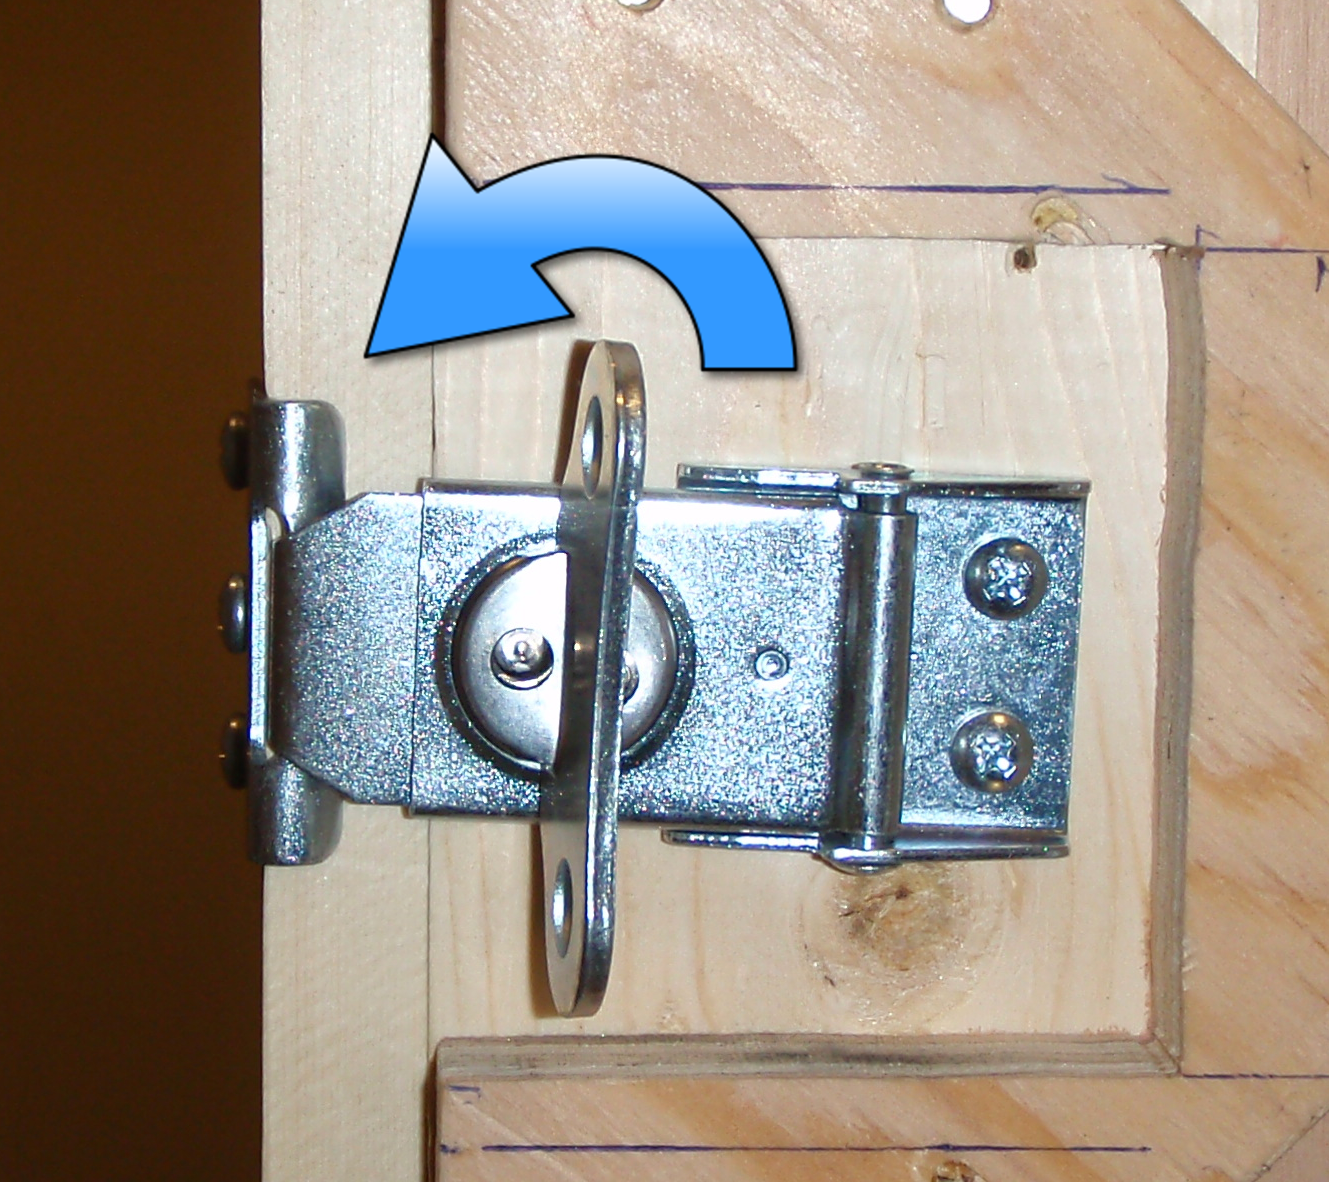
\includegraphics[width=150px]{unlatching.png}
\caption{PR2 crate twist latch.}
\label{fig:unlatch}
\end{figure}

Unlatch the six latches on the front panel and set the panel aside for use
later. Inside the crate is a vaccuum sealed PR2, Figure~\ref{fig:sealPR2},
unlatch and remove the two boards holding the head in place. After the boards
are removed, unlatch all of the latches aroung the bottom of the crate. Make
sure that all of the latch hooks are pushed down and out of the way.

\begin{figure}[h]
\centering
\includegraphics[width=150px]{vaccuumpacked.png}
\caption{PR2 vaccuum sealed in crate.}
\label{fig:sealPR2}
\end{figure}

Now the top of the crate is completely unlatched. {\bf Verify that the two boards holding the head in place have been removed}, and then with two people grab opposite
sides of the crate and slowly walk the crate backwards off the crate
base. Remove all of the plastic wrapping and tape from around the foil vaccuum
wrapping. Once the wrapping is removed cut the foil wrapping about one foot up
from the seam all the way around the base of the robot, this will leave enough
material for repacking the robot if needed. Pull the foil wrapping off and
remove the dessicant bags from around the PR2, Figure~\ref{fig:foamPR2}.

\begin{figure}[h]
\centering
\includegraphics[width=150px]{foamPR2.png}
\caption{PR2 out of foil wrapping.}
\label{fig:foamPR2}
\end{figure}

Slide the foam coverings off of the arms and over the base laser, then remove
the bracing straps on each side of the head, Figure~\ref{fig:head_straps}, using
an 4mm allen wrench. Place the straps and screws in a bag for later use when
repacking the PR2.

\begin{figure}[h]
\centering
\includegraphics[width=150px]{head_strap.png}
\caption{PR2 head straps.}
\label{fig:head_straps}
\end{figure}

Push back the foil wrapping and other materials to reveal the platform in the
base of the crate. In the crate base beneath the PR2 platform is a support board
that must be removed {\bf before} unscrewing the bolts and lowering the platform. Push
the board from one side so that it protudes out the other side and pull it
free. Once the support board is free, use the drill to unscrew the bolts around
the crate base making sure that the two bolts in front of the robot come
completely out of the nuts. Unlatch the board in front of the PR2 base and set
it aside.
